%! alt Triangle ABC with AB = 5, BC = 10 and CA = 13, an example of the condition. Its incircle has centre I and touches BC, CA and AB at Ta, Tb and Tc; the two tangents from A are marked x and the tangent from C along CA is marked z. The median from A to the midpoint Ma of BC is dashed; the centroid G, where the medians meet, lies on it and on the incircle.
%! after_paragraph 1
%! scale 9/20
% The shared preamble of every Cevian figure. pipeline/figures turns these colours into theme-aware paint,
% and refuses any other colour, so draw only with them:
%   figink (lines and labels), figaux (construction lines), figaccent (the object the argument turns on),
%   figtint and figaccenttint (light fills).
\documentclass[border=1.5pt]{standalone}
\usepackage{tkz-euclide}
\definecolor{figink}{RGB}{0,0,0}
\definecolor{figaux}{RGB}{85,85,85}
\definecolor{figaccent}{RGB}{192,57,43}
\definecolor{figtint}{RGB}{221,221,221}
\definecolor{figaccenttint}{RGB}{245,213,208}
% tkz-euclide's defaults draw circles, compasses and marks in 50% grey and fill points with a tint.
\makeatletter
\def\tkz@otherlinecolor{figink}
\def\tkz@euc@circlecolor{figink}
\def\tkz@euc@compasscolor{figink}
\def\tkz@euc@mkcolor{figink}
\def\tkz@mk@fill{figink}
\def\tkz@euc@pointfillcolor{figink}
\makeatother
\tkzSetUpLine[color=figink,line width=.7pt]
\tkzSetUpArc[color=figink,line width=.7pt]
\tkzSetUpCompass[color=figink,line width=.5pt]
\tkzSetUpPoint[color=figink,fill=figink,size=3.1pt]
\tikzset{
  every picture/.style={line cap=round,line join=round,color=figink},
  circle style/.append style={color=figink,line width=.7pt},
  aux/.style={color=figaux,line width=.45pt,dash pattern=on 2.6pt off 2pt},
  key/.style={color=figaccent,line width=1pt},
  mk/.style={color=figink,line width=.5pt},
  lbl/.style={color=figink,inner sep=2.2pt},
  len/.style={color=figink,inner sep=1.5pt,font=\small},
}

\begin{document}
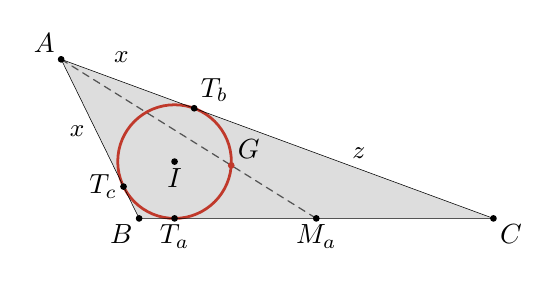
\begin{tikzpicture}
\tkzDefPoint(-0.99000000,2.0204950){A} %! A = (-11/5, 6*sqrt(14)/5)
\tkzDefPoint(0.0,0.0){B} %! B = (0, 0)
\tkzDefPoint(4.5000000,0.0){C} %! C = (10, 0)
\tkzDefPoint(0.45000000,0.72160535){I} %! I = (1, 3*sqrt(14)/7)
\tkzDefPoint(1.1700000,0.67349833){G} %! G = (13/5, 2*sqrt(14)/5)
\tkzDefPoint(0.45000000,0.0){Ta} %! Ta = (1, 0)
\tkzDefPoint(0.69923077,1.3988042){Tb} %! Tb = (101/65, 54*sqrt(14)/65)
\tkzDefPoint(-0.19800000,0.40409900){Tc} %! Tc = (-11/25, 6*sqrt(14)/25)
\tkzDefPoint(2.2500000,0.0){Ma} %! Ma = mid(B, C)
\tkzDefPoint(1.7550000,1.0102475){Mb} %! Mb = mid(C, A)
\tkzDefPoint(-0.49500000,1.0102475){Mc} %! Mc = mid(A, B)
\tkzDefPoint(-0.22500000,2.0475000){Lx} %! Lx = (-0.5, 4.55)
\tkzDefPoint(-0.78750000,1.1025000){Lxx} %! Lxx = (-1.75, 2.45)
\tkzDefPoint(2.7900000,0.83250000){Lzz} %! Lzz = (6.2, 1.85)
%! fact equal(dist(I, Ta), inradius(A, B, C))
%! fact perp(I, Ta, B, C)
%! fact perp(I, Tb, C, A)
%! fact perp(I, Tc, A, B)
%! fact on_segment(Ta, B, C)
%! fact on_segment(Tb, C, A)
%! fact on_segment(Tc, A, B)
%! fact equal(dist(I, Tb), dist(I, Ta))
%! fact equal(dist(I, Tc), dist(I, Ta))
%! fact collinear(G, A, Ma)
%! fact collinear(G, B, Mb)
%! fact collinear(G, C, Mc)
%! fact equal(dist(I, G), dist(I, Ta))
%! fact equal(dist(A, Tc), dist(A, Tb))
%! fact equal(dist(B, Ta), dist(B, Tc))
%! fact equal(dist(C, Ta), dist(C, Tb))
%! example dist(A, B) == 5
%! example dist(B, C) == 10
%! example dist(C, A) == 13
%! example dist(A, Tb) == 4
%! example dist(B, Ta) == 1
%! example dist(C, Ta) == 9
\tkzFillPolygon[color=figtint](A,B,C)
\tkzDrawSegment[aux](A,Ma)
\tkzDrawCircle[key](I,Ta)
\tkzDrawPolygon(A,B,C)
\tkzDrawPoints(A,B,C,I,Ta,Tb,Tc,Ma)
\tkzDrawPoints[color=figaccent,fill=figaccent](G)
\tkzLabelPoint[above left,lbl](A){$A$}
\tkzLabelPoint[below left,lbl](B){$B$}
\tkzLabelPoint[below right,lbl](C){$C$}
\tkzLabelPoint[below,lbl](I){$I$}
\tkzLabelPoint[above right,lbl](G){$G$}
\tkzLabelPoint[below,lbl](Ta){$T_a$}
\tkzLabelPoint[below,lbl](Ma){$M_a$}
\tkzLabelPoint[above right,lbl](Tb){$T_b$}
\tkzLabelPoint[left,lbl](Tc){$T_c$}
\tkzLabelPoint[anchor=center,len](Lx){$x$}
\tkzLabelPoint[anchor=center,len](Lxx){$x$}
\tkzLabelPoint[anchor=center,len](Lzz){$z$}
\end{tikzpicture}
\end{document}
